\documentclass[12pt, a4paper]{article}

% --- Packages ---
\usepackage[margin=1in]{geometry}
\usepackage[T1]{fontenc}
\usepackage{lmodern}              % Scalable Computer Modern fonts
\usepackage{amsmath, amssymb, bm} % Core math packages
\usepackage{graphicx}             % For importing plots
\usepackage{booktabs}             % For professional tables
\usepackage{hyperref}             % For clickable links and citations
\usepackage{setspace}             % For line spacing
\usepackage[numbers,sort&compress]{natbib} % For academic citations
\usepackage{xcolor}               % For highlighting
\usepackage{microtype}            % Better typography

% --- Graphics Path ---
\graphicspath{{paper/figures/}{paper/tex/figures/}{figures/}}

% --- Document Metadata ---
\title{\textbf{Four Findings That Dissolved:\\ A Pre-Registered Audit of a Value-at-Risk Study}}

\author{
    Alvaro Felipe Macias Araya\thanks{AFMA Quant AI Lab, a division of AFMA Ingenier{\'\i}a SpA. All code, data snapshots, pre-registration manifests, and execution ledgers are open-source and publicly verifiable. Correspondence: \href{mailto:amacias@afmaing.cl}{amacias@afmaing.cl}. Web: \href{https://www.afmaing.cl}{www.afmaing.cl}.} \\
    \textit{AFMA Quant AI Lab, AFMA Ingenier{\'\i}a SpA}
}

\date{\today}

\begin{document}

\maketitle

% --- Abstract ---
\begin{abstract}
\noindent A statistically convincing result can be produced by the fitting procedure rather than by the data, and no amount of additional statistical testing will detect this. We document four instances in a single pre-registered study, using as a vehicle the question of whether anchoring a quantile-loss model to a classical Value-at-Risk (VaR) prior improves one-day-ahead forecasts. It does not; that answer is not the contribution. Over eight assets and two quantile levels the study produced four findings, each apparently well supported, and \textbf{all four were subsequently withdrawn}. One fell to a multiplicity correction, one to a power analysis, one to a check of the model's own seed noise---three familiar failures. The fourth was the strongest result in the project, replicated across four runs with a dose--response relationship and a sign test at $p = 5.2 \times 10^{-4}$, and \textbf{it survived every statistical control available}. It dissolved when asked whether the mechanism guaranteed it, at a cost of 28 minutes of validation compute and no test data at all.

\vspace{0.5em}
\noindent We disclose \textbf{1,959 test-set evaluations across 16 asset--level cells and four scoring passes}, with \textbf{zero cells scored only once}, and we reproduce the decisive artefact synthetically with ground truth known: across a ten-point weight grid an anchor carrying \textbf{no information} stabilises the estimator \textbf{at least as much as the true optimum at 9 of 10 weights} (sign test $p = 0.021$) while forecasting materially worse. The two controls that destroyed the two surviving findings---a power calculation and a scale-matched permutation---were also the two cheapest, and a five-paper survey coded against a pre-fixed schema finds neither in use. None of these failures required anyone to behave badly, which is the paper's central argument.
\end{abstract}

\vspace{1em}
\noindent\textbf{Keywords:} Value-at-Risk, Machine Learning Reproducibility, Shrinkage Estimation, Permutation Tests, Model Selection Overfitting, Pre-Registration.

\newpage
\spacing{1.25}

% =========================================================================
\section{Introduction}
% =========================================================================

Machine-learning papers increasingly report statistically significant improvements over classical baselines, supported by careful evaluation protocols and small $p$-values. Comparatively little attention is paid to a different possibility: that a statistically convincing finding can arise from a mechanical property of the fitting procedure itself, and that no amount of additional statistical testing will reveal this, because the mechanism guarantees the result before any data is seen.

This paper is a record of that happening four times in a single pre-registered study.

\textbf{The failures documented here were not produced by bad practice.} None involves fabrication, $p$-hacking, or a protocol anyone would defend as unusual. Each arose inside a design that was pre-registered in advance precisely in order to be careful, and each survived the controls that design specified. That is what makes them worth reporting. A study that fails because its authors cut corners teaches nothing; a study that fails while following the rules identifies a gap in the rules.

\subsection{Where this paper came from}

No one set out to write it. It began as an ordinary applied project with an ordinary ambition: show that anchoring a neural quantile model to a classical VaR prior beats the unanchored model. The intended paper was the one that gets written thousands of times a year---\textit{our method wins, here is the table.}

The starting state is worth describing precisely, because it is unremarkable and that is the point:
\begin{itemize}
    \item The method was called a \textbf{physics-informed neural network}. It was not. No monotonicity or sub-additivity constraint was ever implemented; the mechanism was an $L_2$ penalty toward a rolling parametric prior. The name came from the family of ideas the work was inspired by, and it survived because nothing in the workflow required anyone to check it against the code. \textbf{The paper's own title was wrong before any result was.}
    \item Hyper-parameters were chosen by running the pipeline and looking at the output. There was no validation block, so they were selected on the test set.
    \item Each configuration ran on \textbf{one seed}.
    \item Models were ranked on breach counts and ``capital reserved'' rather than on a strictly consistent loss.
    \item The GARCH benchmark carried a standardized-$t$ scaling error that inflated its VaR by $\nu/(\nu-2)$---that is, \textbf{the baseline we were beating was handicapped} (Section~\ref{sec:defects}).
\end{itemize}

Every item on that list is a decision someone made while trying to do good work, and none would have been caught by peer review of the resulting manuscript, because none is visible in a manuscript. Fixing them was not a matter of discovering misconduct. It was a matter of a protocol asking questions the original workflow had no place to put.

What followed is the substance of this paper: each correction moved the result toward the null, and after four of them there was no result left. The four withdrawals below are not a catalogue of things other researchers do wrong. \textbf{They are what one careful project looked like when it was finally instrumented well enough to see itself.}

\subsection{Setting and scope}

\textbf{The vehicle is a Value-at-Risk study}, chosen because it is a domain with well-established baselines \citep{engle1982, bollerslev1986, koenker1978}, a strictly consistent scoring function \citep{gneiting2011, fissler2016}, and standard backtests \citep{kupiec1995, christoffersen1998}---an unusually favourable setting for detecting a spurious result. The question was narrow: does an $L_2$ penalty anchoring a quantile-loss model to a classical VaR prior improve one-day-ahead forecasts? The answer is no. That answer is not the contribution, and readers interested in VaR modelling specifically will find Section~\ref{sec:limitations} disappointing by design.

A survey of \textbf{five} machine-learning VaR papers \citep{petnehazi2019, lux2020, taylor2019}, each read in full and coded against a schema fixed before any paper was read, locates the gap more precisely. Practice in this literature is \textbf{heterogeneous, and no paper in the sample is careless.} Two use a held-out selection block; one selects on a strictly consistent loss and ensembles twenty networks; one applies Hansen's SPA test \citep{hansen2005} and then explicitly downgrades its own $p$-values for multiplicity; all five gate on coverage.

Across all five, however: \textbf{test-set reuse is never counted, no power analysis appears, and none is pre-registered.} Inter-seed dispersion is never reported in the four where the question applies. And \textbf{four of five rank models on something other than a strictly consistent scoring function}---exceedance rates, Lopez-family losses, or in one case the $p$-value of a conditional-coverage test used simultaneously to select and to evaluate.

The controls this field has institutionalised are not the controls that defeated this study. A convenience sample of five cannot establish a base rate and we do not claim it does; by the standard Section~\ref{sec:finding2} applies to our own nulls, it is an illustration.

\paragraph{Contributions.}
\begin{enumerate}
    \item A pre-registered VaR study reporting a complete null, with dated amendments including several that weakened the authors' own position. Pre-registration remains rare in this domain: as of July 2023 \textbf{$\le 1\%$ of economics journals} had adopted the registered-report format \citep{lin2024, arpinon2023}.
    \item \textbf{Four failure modes observed in a single pre-registered study}, with the control that detects each and its cost. We claim instances, not coverage: one study cannot establish a taxonomy and we do not present one.
    \item A demonstration---analytical and synthetic, with ground truth known---that \textbf{shrinkage-induced stability is not evidence of a good prior}, together with a scale-matched permutation control that separates the two for minutes of compute. \textbf{Neither the mechanism nor the control is new}: the mechanism is Stein/ridge shrinkage \citep{stein1956, james1961, hoerl1970}, and the control is a restricted randomization test with precedents in statistics, machine learning and econometrics \citep{fisher1935, pitman1937, ojala2010, zhang2017, adebayo2018, bertrand2004}. What we document is that the artefact is \textit{reportable as an empirical finding}, survives a pre-registered protocol with a dose--response and $p = 5.2 \times 10^{-4}$---and that we located no prior application of the control to a stability claim.
    \item An append-only \textbf{test-touch ledger} that makes evaluation reuse countable rather than reconstructible after the fact.
\end{enumerate}

% =========================================================================
\section{Setup}
% =========================================================================

\paragraph{Question.} Does an $L_2$ penalty pulling a quantile forecast toward a classical VaR prior (rolling Normal $\mu - z\sigma$, or rolling historical quantile) improve out-of-sample pinball loss relative to the identical unanchored model?

\paragraph{The estimator nests its own baseline.} The anchor weight grid includes zero, so the anchored specification \textit{contains} the unanchored one. It therefore cannot be worse by construction; it can only lose through validation-selection error (Section~\ref{sec:finding2}).

\paragraph{Data.} Eight instruments spanning equity index (\textsf{\textasciicircum GSPC}), single names (\textsf{TSLA}, \textsf{NVDA}, \textsf{SQM}), crypto (\textsf{BTC-USD}), metals (\textsf{HG=F}), energy (\textsf{CL=F}) and FX (\textsf{CLP=X}). Ten-year frozen snapshots with SHA-256 manifests, verified on every load. Daily log returns.

\paragraph{Protocol.} Chronological TRAIN / VAL / TEST; monthly refit on an expanding window with warm start; $\ge 10$ seeds per specification reported as median and IQR; pinball loss for ranking; Kupiec \citep{kupiec1995} and Christoffersen \citep{christoffersen1998} as a coverage gate; Diebold--Mariano \citep{diebold1995} with HAC errors for pairs; Hansen's Model Confidence Set \citep{hansen2011} across the ladder.

\paragraph{Primary evidence set.} Only two cells had ever been scored before the main panel (\textsf{\textasciicircum GSPC} at both levels and \textsf{BTC-USD} at $\alpha = 0.05$, during debugging). Excluding them leaves \textbf{13 cells, 7 tickers, 26 comparisons} of genuine first contact. The exclusion criterion is file timestamps, independent of any result; the check in Section~\ref{sec:checks} shows that it moves both headline numbers \textit{against} the study's own thesis.

% =========================================================================
\section{Four Findings and Their Withdrawals}
% =========================================================================

The four withdrawals are not equivalent, and presenting them as a flat list would obscure the one that matters.

\textbf{The first three are familiar.} Multiplicity, insufficient power, and effects smaller than the estimator's own noise are textbook failure modes; each has a named remedy, each remedy is uncontroversial, and a sufficiently careful referee would ask for all three \citep{harvey2016, button2013, summers2021}. They are reported here because they occurred \textit{despite} pre-registration, and because their costs are worth tabulating---but a reader who knows the literature will find nothing structurally new in Sections~\ref{sec:finding1} to \ref{sec:finding3}. They are the price of admission.

\textbf{The fourth is not.} It is the only one where the finding survived every statistical control available---multiplicity correction, dose--response, replication across four runs, a sign test at $p = 5.2 \times 10^{-4}$---and dissolved only when asked a question that is not statistical at all: \textit{does the mechanism guarantee this result regardless of whether the hypothesis is true?} Sections~\ref{sec:finding4} and \ref{sec:synthetic} are the substance of the paper; Sections~\ref{sec:finding1} to \ref{sec:finding3} establish that the study was careful enough for Section~\ref{sec:finding4} to be surprising.

\subsection{``Anchoring improves out-of-sample loss'' --- multiplicity}
\label{sec:finding1}

Three of 26 comparisons reject at 5\% uncorrected. \textbf{One survives Holm.} More seriously, by the time we reported this the test block had been scored four times, so no comparison retains out-of-sample status \citep{white2000}.

\vspace{0.5em}
\noindent\textit{Control: a multiplicity correction and a count of test-set passes. Cost: free.}

\subsection{``Weight selection is indistinguishable from chance'' --- power}
\label{sec:finding2}

Of 16 comparisons where validation selected a non-zero weight, \textbf{6 (37.5\%) were worse than $w = 0$} on the evaluation block. Binomial $p = 0.45$ against a coin flip; 95\% CI $[0.15, 0.65]$. We initially reported this as evidence that the selection signal is noise.

It is not. At $n = 16$ the design detects a proportion only below \textbf{0.147} or above \textbf{0.853}. Power against the observed effect is \textbf{9.5\%}. Reaching 80\% power would need \textbf{125 comparisons}. A selection procedure with a genuinely useful 30\% error rate would have been missed 91\% of the time \citep{button2013}.

The correct statement is \textit{undetermined}, not \textit{chance}. We also retract our earlier framing of four configurations as independent replications: they share assets and periods.

\textbf{And ``undetermined'' is still not the whole answer.} \citet{cawley2010} established that a model-selection criterion is itself an estimator with a variance, and that optimising it over a finite sample \textbf{over-fits the criterion} exactly as training over-fits the data \citep{varma2006, bengio2004}. Two of their findings apply directly:
\begin{itemize}
    \item They deliberately construct \textit{``a split-sample based model selection strategy with a relatively high variance, \textbf{due to the limited size of the validation set}''}---which is our design, not a pathological case. Enlarging the validation block tightens the selected hyper-parameter around the optimum; ours was fixed and short.
    \item More seriously: \textit{``the effects of this form of over-fitting are often of \textbf{comparable magnitude to differences in performance between learning algorithms}.''} Our observed anchoring edges are 1--8\% of the loss level. \textbf{If selection over-fitting operates at the same scale as the effect being measured, the comparison was conducted inside the noise floor of its own selection step}---a stronger and more specific statement than ``underpowered.''
\end{itemize}

They also observe that the criterion surface is often \textit{``a broad valley,''} so a badly chosen hyper-parameter can still generalise adequately \citep{bergstra2012}. That is a better account of our 37.5\% than the one we first gave: not that selection carries no signal, but that the surface is flat and the block is short.

Their prescribed remedy---\textit{``evaluation \dots should always involve multiple partitions of the data to form training/validation and test sets''}---is only partly available here, because the data are time series and shuffling would leak. The available version is multiple \textbf{chronological} origins. We did not run them. That is a limitation, not a defence.

\vspace{0.5em}
\noindent\textit{Control: a power calculation. Cost: free. Never performed until a reviewer demanded it. The relevant literature is from 2010 and we did not read it until after the result.}

\subsection{``Higher capacity hurts accuracy'' --- the model's own noise}
\label{sec:finding3}

An 8,641-parameter MLP lost to a 4-parameter linear model in 4 of 5 assets. \textbf{Zero of the five gaps exceed the combined inter-seed IQR of the two models being compared.} The MLP also inherited its learning rate and epoch budget from the linear model and was never tuned; convergence was not recorded and so is unfalsifiable.

\vspace{0.5em}
\noindent\textit{Control: compare effect sizes to the models' own seed dispersion. Cost: free.}

\subsection{``Anchoring stabilises the estimator'' --- tautology}
\label{sec:finding4}

This was the strongest result in the project. Across four runs the anchored estimator had lower inter-seed IQR in 19/20, 21/23, 25/27 and \textbf{15/16} comparisons (primary set: $p = 5.2 \times 10^{-4}$, median ratio \textbf{13.5$\times$, 95\% CI 4.6--20.7}, $n = 16$), with a clean dose--response between the selected weight and the effect: \textbf{Spearman $\rho = +0.585$, $p = 4.1 \times 10^{-9}$, $n = 85$}.

\begin{figure}[htbp]
    \centering
    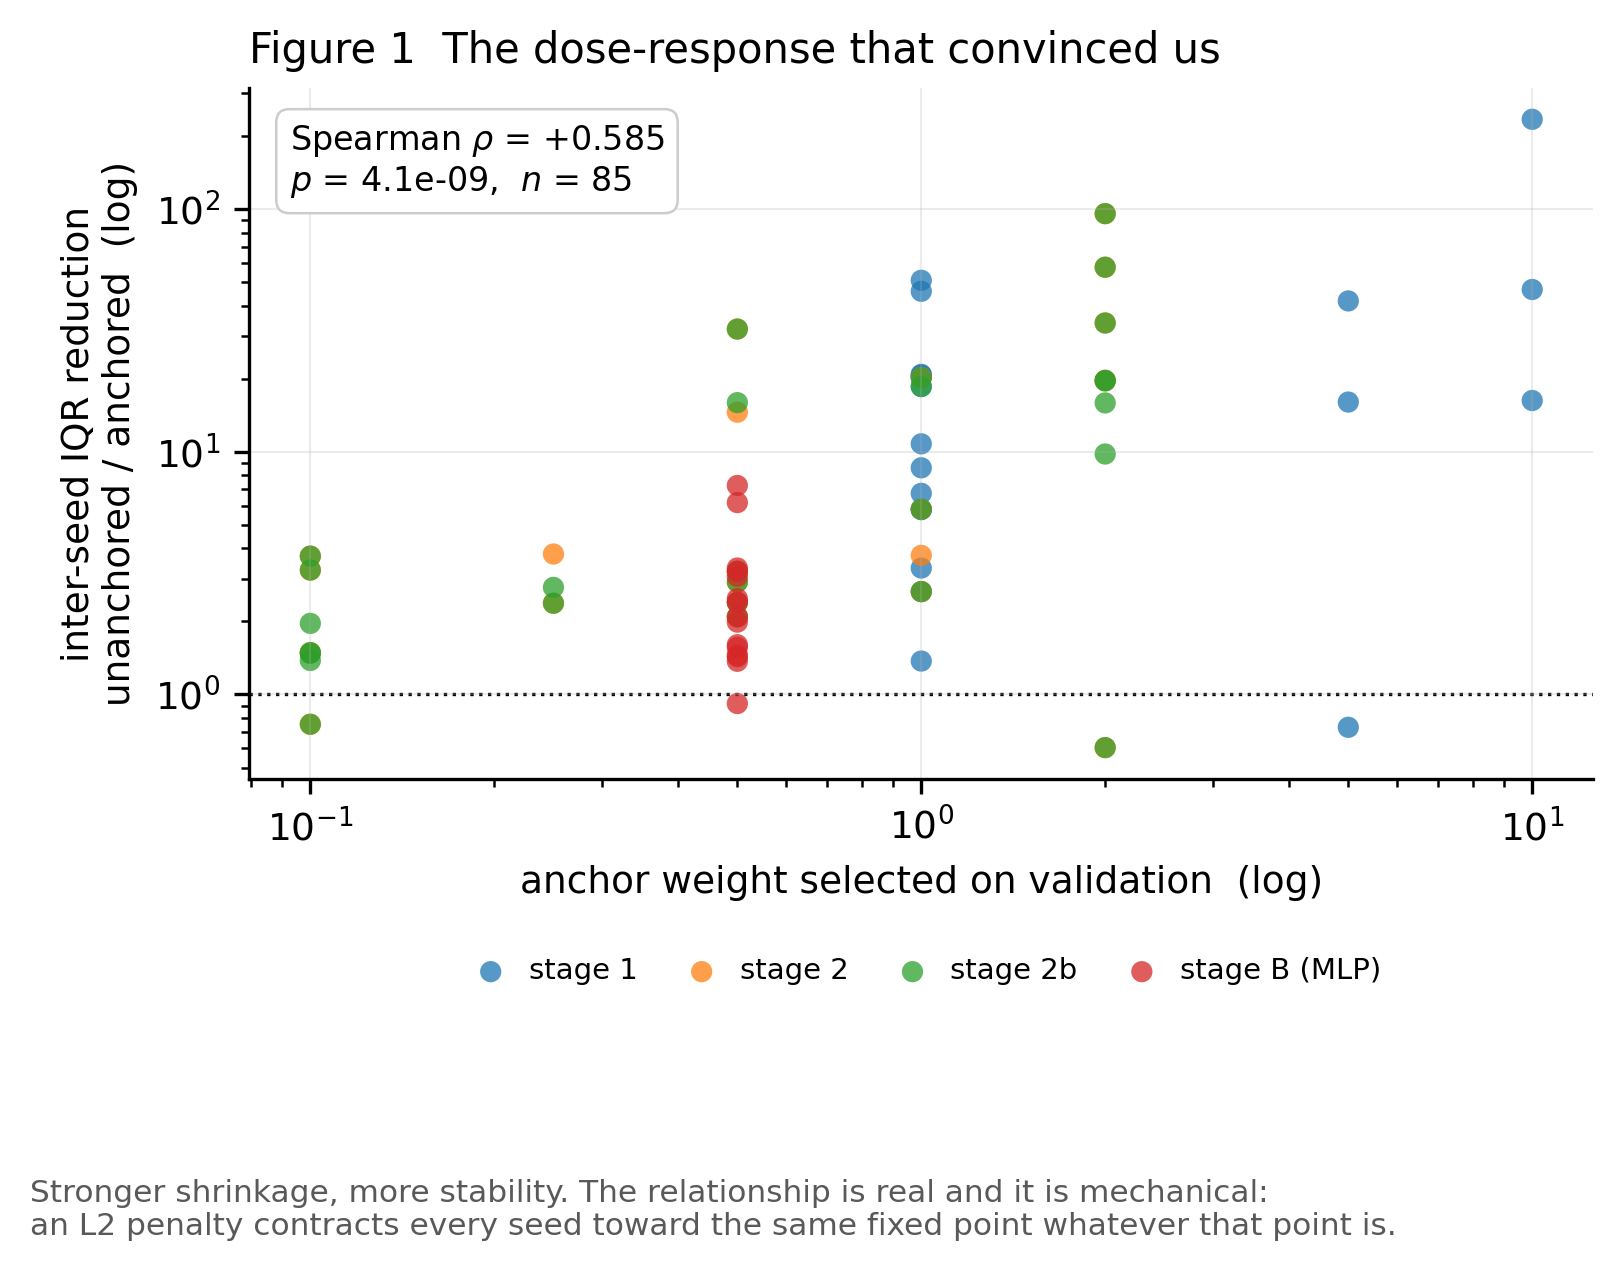
\includegraphics[width=0.78\textwidth]{figure1_dose_response.png}
    \caption{\textbf{The dose--response that convinced us.} Scatter plot of anchor weight $w$ against the inter-seed IQR ratio (unanchored IQR $\div$ anchored IQR), pooled across all four runs ($n = 85$, Spearman $\rho = +0.585$, $p = 4.1 \times 10^{-9}$). It is an algebraic artefact of $L_2$ shrinkage toward a fixed target.}
    \label{fig:dose_response}
\end{figure}

Figure~\ref{fig:dose_response} is reproduced here because it is persuasive. It is the evidence that convinced us, pooled across all four runs, and it is an artefact. A referee who would have accepted this plot should note that acceptance is the failure mode under discussion.

An $L_2$ penalty pulls every seed toward the \textit{same fixed target}. As the weight grows all seeds converge on that target and inter-seed dispersion goes to zero \textbf{by construction}---whatever the target is. The dose--response we took as corroboration is the signature of the artefact.

\paragraph{The control.} Re-run with the real prior \textbf{permuted in time}: identical mean, standard deviation and marginal distribution; correlation with tomorrow's absolute return 0.0007 versus 0.041. Matched on magnitude, stripped of information.

\begin{table}[htbp]
\centering
\small
\caption{\textbf{Paired comparison: real prior vs. shuffled prior.} Ratio of unanchored to anchored seed-IQR across three assets and two weights.}
\label{tab:permuted_control}
\begin{tabular}{lccc}
\toprule
\textbf{Ticker} & \textbf{Weight ($w$)} & \textbf{Real Prior} & \textbf{Shuffled Prior} \\
\midrule
\textsf{NVDA}     & 0.5 & 1.55$\times$  & 1.49$\times$ \\
\textsf{NVDA}     & 1.0 & 2.25$\times$  & \textbf{2.91$\times$} \\
\textsf{SQM}      & 0.5 & 0.76$\times$  & 0.63$\times$ \\
\textsf{SQM}      & 1.0 & 1.33$\times$  & 1.15$\times$ \\
\textsf{\textasciicircum GSPC} & 0.5 & 3.05$\times$  & \textbf{3.10$\times$} \\
\textsf{\textasciicircum GSPC} & 1.0 & 12.47$\times$ & \textbf{16.76$\times$} \\
\bottomrule
\end{tabular}
\end{table}

The uninformative prior matches or beats the real one in 3 of 6 cells (Table~\ref{tab:permuted_control}); \textbf{Wilcoxon $p = 0.844$}. Bootstrapped over comparisons, the two are indistinguishable: real prior \textbf{1.9$\times$ (95\% CI 1.0--7.8)} against shuffled \textbf{2.2$\times$ (95\% CI 0.9--9.9)}. The intervals overlap almost entirely, which is a more informative statement of the null than the rank test alone.

\vspace{0.5em}
\noindent\textit{Control: shrink toward a scale-matched nonsense target. Cost: 28 minutes, validation only, zero test-set evaluations.}

\paragraph{A trap.} Pooling all controls gives 1.32$\times$ against 2.36$\times$ for informative priors, which looks like a genuine gap. It is produced entirely by a control shrinking toward an off-scale target, which fights the data rather than shrinking within it. Only the \textbf{scale-matched} comparison is diagnostic, and it is null. Reporting the aggregate would have preserved the claim.

\textbf{This is a restricted randomization test, and we should have known that before running it.} The requirement we arrived at by tripping over the trap above---that the permuted target must preserve the properties irrelevant to the hypothesis and destroy only the one under test---is stated directly by \citet{ojala2010}, whose second permutation test permutes features within classes for exactly this reason: \textit{each randomization method entails a certain null distribution, that is, which properties of the original data are preserved.} An off-scale control induces a different null and is therefore not diagnostic. We report the sequence honestly---we found the constraint empirically and located its name afterwards---because the control is more credible with a seventy-year lineage \citep{fisher1935, pitman1937} than as an invention of ours.

\subsection{The artefact isolated: a synthetic demonstration}
\label{sec:synthetic}

One case does not establish that the artefact is general. It is therefore reproduced where the ground truth is known and nothing is estimated from markets.

\paragraph{Setup.} $y = X\beta + \epsilon$, $\epsilon \sim \mathcal{N}(0,1)$, so the optimal linear $\alpha$-quantile is exactly $X\beta + z_\alpha$ and is available in closed form. Fitting descends $\text{pinball}(y - X\theta) + w \|\theta - a\|^2$ from random initialisations under a \textbf{finite step budget}---the condition that produces seed dispersion in the first place, and the condition the real study was under via early stopping. Three anchors: the \textbf{true} optimum; a \textbf{scale-matched nonsense} vector with identical norm pointing elsewhere; and zero.

\paragraph{Analytically,} the penalty's gradient is $2w(\theta - a)$, so each gradient descent step contracts the gap between two runs that differ only in initialisation:
\begin{equation}
    \text{spread}_T \sim \text{spread}_0 \cdot (1 - 2\eta w)^T
\end{equation}
This depends on weight $w$, learning rate $\eta$, and step count $T$. \textbf{It contains no reference to target $a$.} Shrinking toward the truth and shrinking toward nonsense contract inter-seed dispersion by the exact same factor.

\paragraph{Numerically,} over a ten-point log-spaced weight grid with 40 seeds per cell (pure NumPy, 22 seconds), results are displayed in Table~\ref{tab:synthetic_grid}.

\begin{table}[htbp]
\centering
\small
\caption{\textbf{Synthetic demonstration across ten weights.} Ratio of unanchored to anchored seed-IQR for true vs. nonsense anchors (40 seeds per cell).}
\label{tab:synthetic_grid}
\begin{tabular}{cccc}
\toprule
\textbf{Weight ($w$)} & \textbf{True Anchor} & \textbf{Nonsense Anchor} & \textbf{Nonsense $\div$ True} \\
\midrule
0.0005 & 1.05$\times$  & 1.09$\times$  & 1.03 \\
0.0009 & 1.10$\times$  & 1.12$\times$  & 1.02 \\
0.0016 & 1.13$\times$  & 1.17$\times$  & 1.04 \\
0.0029 & 1.17$\times$  & 1.23$\times$  & 1.05 \\
0.0053 & 1.26$\times$  & 1.28$\times$  & 1.02 \\
0.0095 & 1.31$\times$  & 1.21$\times$  & \textbf{0.93} \\
0.0171 & 1.51$\times$  & 1.67$\times$  & 1.11 \\
0.0308 & 2.39$\times$  & 6.09$\times$  & 2.55 \\
0.0555 & 5.46$\times$  & 17.81$\times$ & 3.26 \\
0.1000 & 50.40$\times$ & 79.23$\times$ & 1.57 \\
\bottomrule
\end{tabular}
\end{table}

\textbf{Paired at each weight}, the uninformative anchor stabilises \textbf{at least as much as the true optimum at 9 of 10 weights} (sign test \textbf{$p = 0.021$}), with a median relative ratio of \textbf{1.04 (95\% CI 1.0--1.8)}. The dose--response is emphatic and holds for every anchor (Spearman $\rho = \mathbf{+0.974}$, $p = 1.3 \times 10^{-19}$, $n = 30$), reproducing the pattern we had taken as corroboration in the real study ($\rho = +0.585$).

Loss moves the other way: the true anchor improves out-of-sample loss, the nonsense anchor degrades it. \textbf{Stability tracks the penalty; usefulness tracks the target. They are different axes, and only the second is evidence.}

\begin{figure}[htbp]
    \centering
    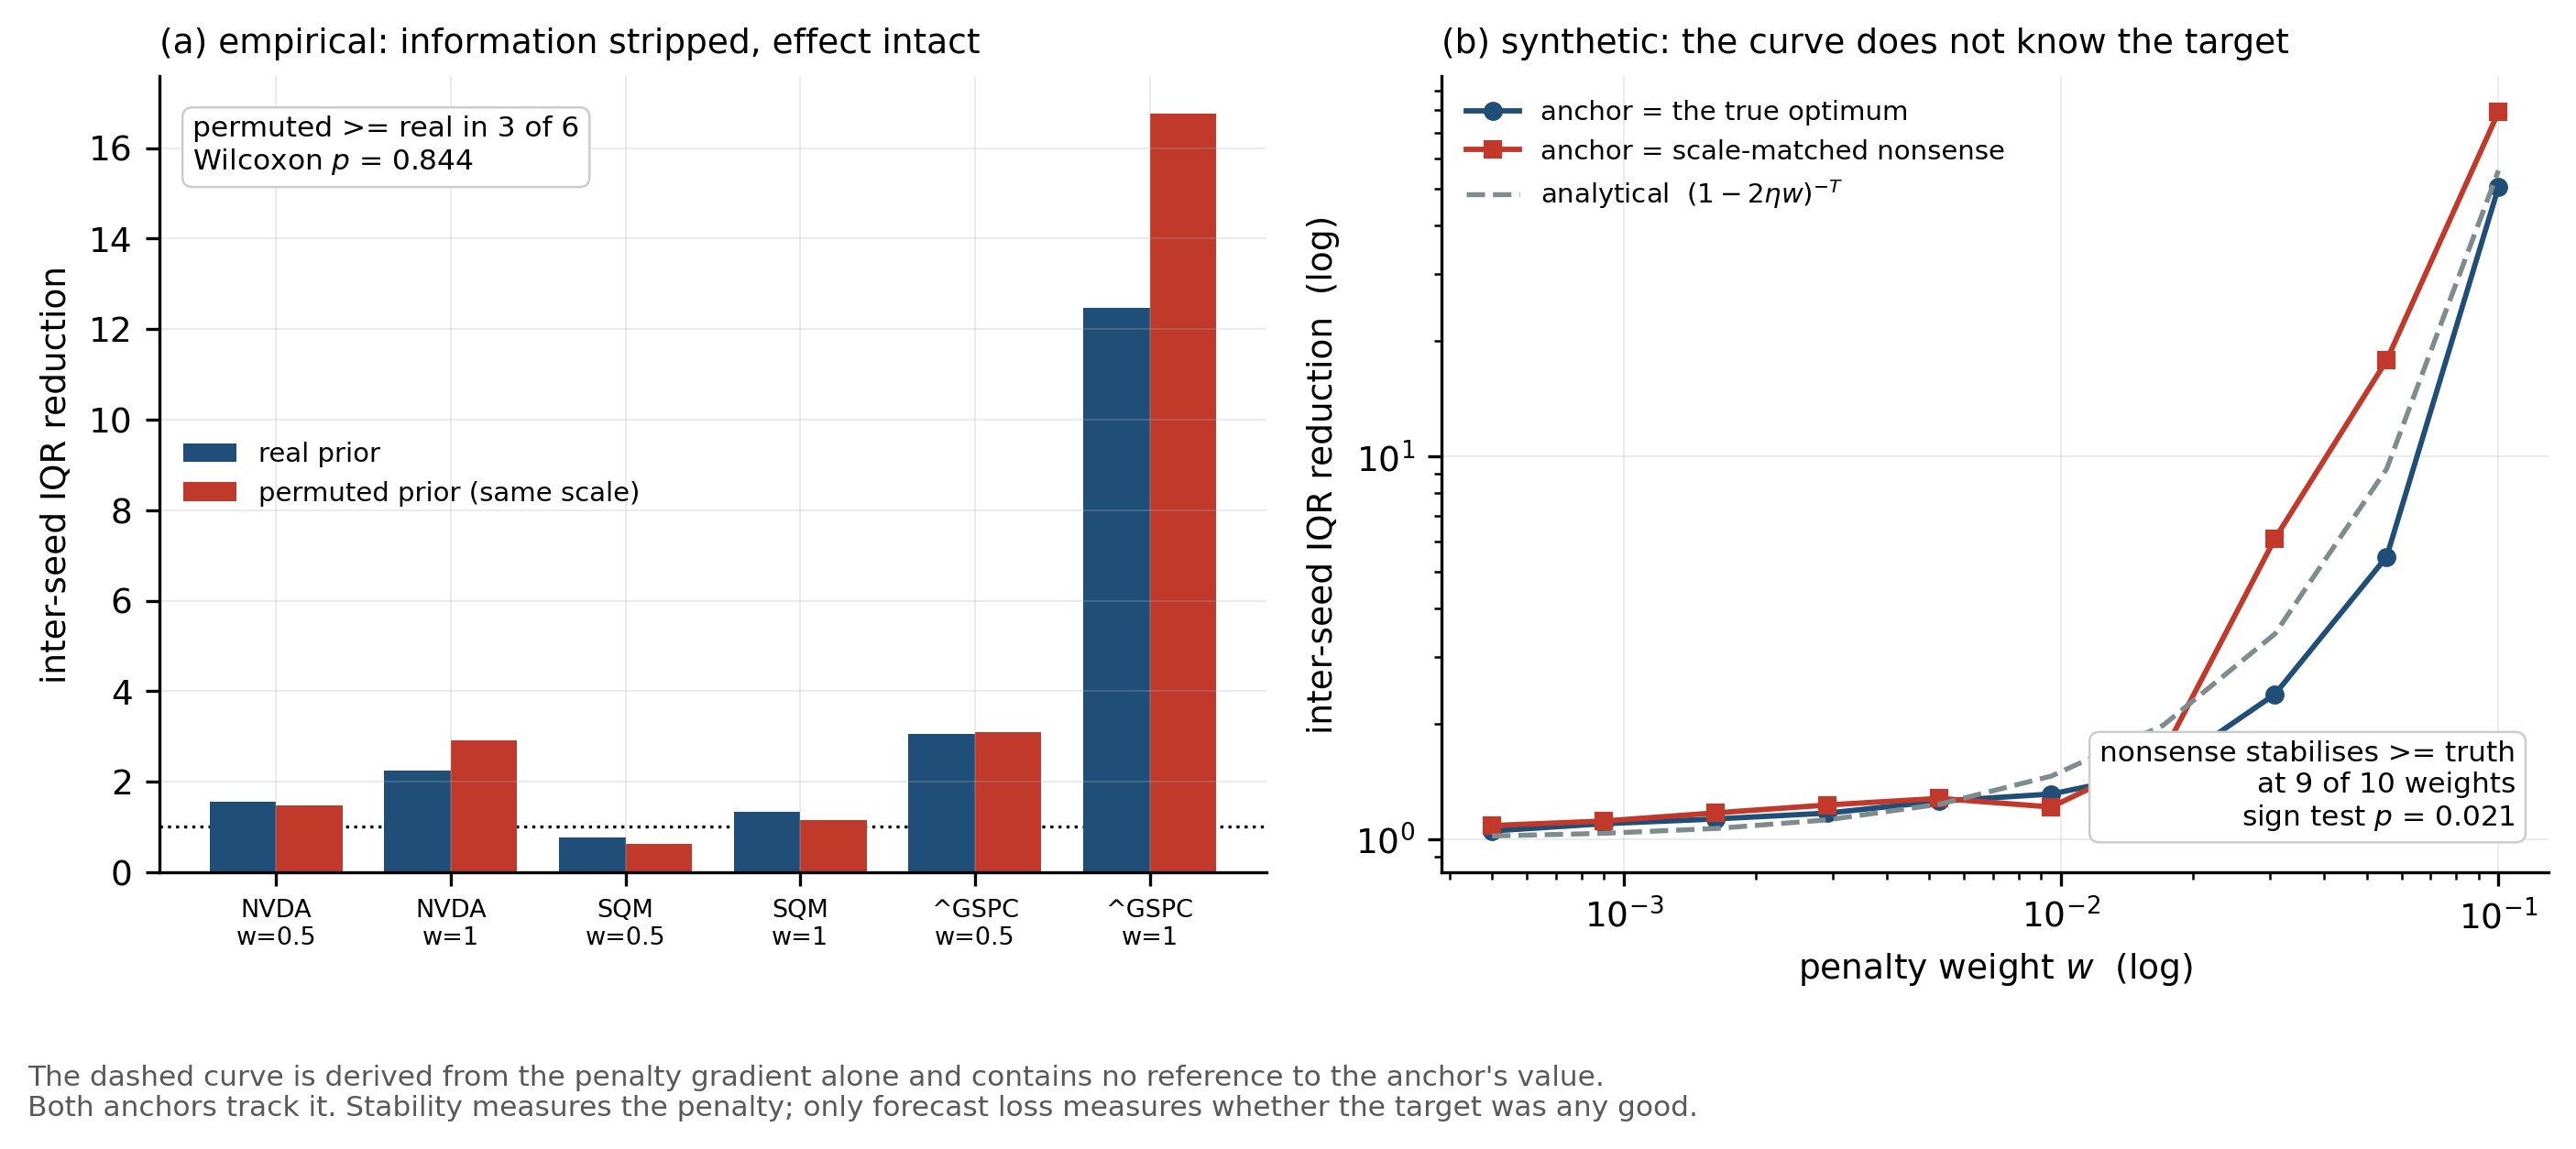
\includegraphics[width=0.92\textwidth]{figure2_control.png}
    \caption{\textbf{Figure 1 with a control.} \textit{Panel (a):} empirical comparison against a prior permuted in time; the stability effect is unchanged. \textit{Panel (b):} overlay of the analytical contraction $(1 - 2\eta w)^{-T}$ derived purely from the penalty gradient. Both the true and the nonsense anchor track it exactly.}
    \label{fig:control_overlay}
\end{figure}

Figure~\ref{fig:control_overlay} displays this synthesis. Panel (a) repeats the empirical comparison against a prior permuted in time; the effect is unchanged. Panel (b) overlays the analytical contraction $(1 - 2\eta w)^{-T}$---a curve derived from the penalty gradient alone, which contains no reference to the anchor's value. Both the true and the nonsense anchor track it. The dashed line is the whole argument: it predicts the data without knowing what the data was shrunk toward.

\paragraph{Generalisation.} For any regularised estimator, stability under a shrinkage penalty is not evidence that the shrinkage target is good. The mechanism is Stein/ridge shrinkage \citep{stein1956, james1961, hoerl1970} and is not itself new; what we document is that it is \textbf{reportable as an empirical finding}, that it survives a pre-registered protocol with a dose--response and $p = 5.2 \times 10^{-4}$, and that a scale-matched permuted control detects it for minutes of compute.

\textbf{Nothing about that control is ours.} It is a restricted randomization test \citep{fisher1935, pitman1937, ojala2010}, and the move it makes---randomize the input a claim depends on and check whether the claim survives---is the move behind the random-label experiment of \citet{zhang2017}, the model- and data-randomization sanity checks of \citet{adebayo2018}, and the placebo laws of \citet{bertrand2004}, who found conventional difference-in-differences standard errors significant at 5\% for up to 45\% of interventions that never happened. Four literatures already treat this as routine \citep{abadie2010, bailey2014deflated}.

What we could not find is an instance applied to a \textbf{stability} claim rather than an accuracy or treatment-effect claim. We state that as a search null and not as a gap: by the standard Section~\ref{sec:finding2} applies to this study's own nulls, failing to find something is not evidence it is absent. We offer Section~\ref{sec:finding4} as a template, not as a method---and the appropriate conclusion is that a control already standard in four fields should be applied in a fifth, which is a much weaker and much more defensible claim than novelty.

\paragraph{The practice we set out to criticise turns out to be handled correctly where it originates.} We expected to find regularisers proposed as remedies for run-to-run variance, with the resulting stability offered as evidence of quality. The first half is true---\citet{bhojanapalli2021} propose entropy regularisation and co-distillation precisely to reduce prediction \textit{churn} between independently trained models \citep{summers2021}. The second half is false. They report accuracy beside churn in every table, measure churn across independent runs of the whole procedure rather than between the two coupled models (the circular version), disclose the calibration cost, include a fully deterministic run at \textbf{churn 0.00} whose accuracy is indistinguishable from baseline, and state the point of our Section~\ref{sec:synthetic} in prose: \textit{multiple runs of a deterministic learning algorithm produce models with zero churn, independent of their accuracy.}

We report this because it weakens the section. It also sharpens it. \textbf{Our error was not reporting stability; it was inferring from stability a conclusion about the target.} For \citet{bhojanapalli2021} reduced churn \textit{is} the objective---a deployment requirement in its own right---and accuracy is checked separately to confirm nothing was traded away. We instead used stability as evidence that the anchor carried risk information, which is a claim about the target that no property of the penalty can support \citep{madani2004}.

The failure is therefore not a field's carelessness. It is what happens when a concept crosses domains and its controls do not travel with it. The one documented instance we have of the inference being made explicitly is in a VaR paper \citep{petnehazi2019}, which offers \textit{``consistently lower standard deviation than the benchmark methods\dots which also justifies that this one produces the highest quality VaR estimates''} with no matched control. We made the same move, in the same domain, four years later.

% =========================================================================
\section{Disclosure}
% =========================================================================

From the append-only ledger, not a hand count:

\begin{table}[htbp]
\centering
\small
\caption{\textbf{Test-touch disclosure ledger.}}
\label{tab:ledger}
\begin{tabular}{lc}
\toprule
\textbf{Quantity} & \textbf{Value} \\
\midrule
Test-set evaluations               & \textbf{1,959} \\
Asset--level cells                 & 16 \\
Maximum scoring passes on one cell & \textbf{4} \\
Cells scored exactly once          & \textbf{0} \\
\bottomrule
\end{tabular}
\end{table}

Design choices between passes---weight grid, selection rule, architecture, asset subset---were informed by the previous pass's outcomes. Per our own protocol the honest description is that this project has several validation blocks and \textbf{no test set}.

The ledger figure exceeds the 1,899 we first reconstructed from run manifests: two early debugging runs appear in no manifest. That 60-evaluation gap is precisely what an append-only ledger exists to prevent, and it was found only because we built one.

% =========================================================================
\section{Three Defects, All in the Same Direction}
\label{sec:defects}
% =========================================================================

This section is not a confession, and should not be read as one. Each defect below is the kind that a competent implementation produces and a code review passes: a plausible convergence rule, a NaN-handling choice, an unguarded edge case. What is worth attention is not that they occurred but \textit{where they were found}---all three surfaced when an unrelated check failed, none when a result that looked correct was audited.

\begin{enumerate}
    \item \textbf{Early stopping.} The rule halted when consecutive epochs changed by $< 10^{-6}$. Pinball loss on a linear model is piecewise linear and plateaus; the $L_2$ anchor makes the objective smooth. The anchored model trained roughly 42$\times$ more epochs per block. \textit{The anchor bought training, not information.}
    \item \textbf{Unequal training rows.} Rows with an undefined prior were dropped only when an anchor was active, giving $w = 0$ about 252 extra rows. The weight grid was not comparing like with like.
    \item \textbf{A Diebold--Mariano exception} on identical forecasts crashed 8 of 16 cells---exactly those where validation had switched the anchor \textit{off}, the most informative outcome available.
\end{enumerate}

Each defect, before correction, favoured the hypothesis under test.

\textbf{We must be careful here, because this is exactly the kind of claim this paper is about.} Three of three in the same direction is \textbf{$p = 0.125$} one-sided under independent signs. By our own standard in Section~\ref{sec:finding2}---where 6/16 at $p = 0.45$ was ruled insufficient---$n = 3$ cannot support a conclusion, and we do not draw one.

What we offer instead is a mechanism worth testing by someone with a larger sample: \textit{a defect that contradicts your hypothesis gets investigated; one that confirms it gets shipped.} Each of these three was found only because an unrelated check failed, not because anyone audited a result that looked right. That asymmetry in scrutiny is measurable in principle---count, across a corpus of projects, the direction of defects found before versus after publication---and we suggest it be measured rather than asserted \citep{simmons2011, gelman2014}.

\subsection{A fourth class of defect, found by checking the bibliography}

Twenty citations in this paper were stated from standing knowledge---author, year, venue---pending verification against the published record. Checking all twenty found \textbf{five errors} (Table~\ref{tab:citation_errors}).

\begin{table}[htbp]
\centering
\small
\caption{\textbf{Citation verification pass.} Errors identified when checking 20 unverified references against the published record.}
\label{tab:citation_errors}
\begin{tabular}{lp{10cm}}
\toprule
\textbf{Citation} & \textbf{The Error} \\
\midrule
Fisher (1935)         & Given as ``ch.~21''; the randomization test is \textbf{\S21 within Chapter III}. \\
Gelman \& Loken       & Cited as a 2013 working paper; published as \textbf{2014, \textit{American Scientist} 102(6)}. \\
Madani et al.\ (2004) & Wrong authors (\textit{Pena \& Hsu} $\to$ \textbf{Pennock \& Flake}); \textbf{the claim about it was backwards}. \\
Taylor (2019)         & Described as a quantile neural network; it is \textbf{semiparametric asymmetric-Laplace}. \\
Lin et al.            & Dated 2023; published in \textbf{2024}, \textit{Scientometrics} 129(4). \\
\bottomrule
\end{tabular}
\end{table}

\textbf{Four of the five were inherited from other people's descriptions of a source, or from a metadata string, rather than from the source itself.} A citation copied from a citation is not a verified citation, and the resulting error rate---five in twenty---is higher than we would have guessed before measuring it.

The Madani case is the one worth dwelling on. It had been recorded, from a mention inside another paper, as a probable early instance of stability being used as a quality signal---that is, as \textit{evidence for this paper's argument}. Reading it showed the opposite: they derive bounds relating prediction disagreement to generalization error rather than assuming the relationship. \textbf{Left unchecked it would have entered the paper as a fabricated ally.}

There is a coda we report without irony. The Lin et al.\ article \citep{lin2024}---the one whose date we got wrong---is a bibliometric study whose authors follow a method of their own devising called \textit{precise citation}, having previously published a paper on citation accuracy. \textbf{It carries a published correction stating that its own citation information for Table~1 was incorrect.}

If a paper about citation accuracy, by authors who wrote a paper about citation accuracy, needs a citation correction, then five in twenty is not a story about anyone being careless. It is a base rate. And the only defence against a base rate is a procedure, not an intention---which is the same conclusion Section~\ref{sec:finding4} reached by a different route.

% =========================================================================
\section{Checks on This Study's Own Analysis}
\label{sec:checks}
% =========================================================================

The primary evidence set is a post-hoc subset, which invites the obvious objection. Its selection criterion is mechanical (file timestamps) and result-independent, and it moves both headline numbers \textit{against} the hypothesis under test (Table~\ref{tab:checks}).

\begin{table}[htbp]
\centering
\small
\caption{\textbf{Internal consistency checks.} Sensitivity of headline metrics to the post-hoc evidence subset.}
\label{tab:checks}
\begin{tabular}{lccc}
\toprule
\textbf{Metric} & \textbf{Full Stage 1} & \textbf{First-Touch Subset} & \textbf{Direction} \\
\midrule
Selection error             & 45\%   & \textbf{38\%}  & Further from 50\% (weakens null) \\
Seed-IQR reduction (median) & 16.1$\times$ & \textbf{13.5$\times$} & Smaller (weakens stability) \\
\bottomrule
\end{tabular}
\end{table}

\paragraph{Residual contamination.} The seven first-touch assets were never \textit{scored} before, but the code that scored them was revised after inspecting \textsf{\textasciicircum GSPC}'s output---that is how defects 1 and 2 were found. This is weaker than a pristine holdout and we say so rather than claiming otherwise.

% =========================================================================
\section{The Taxonomy}
% =========================================================================

Table~\ref{tab:taxonomy} summarises the controls deployed, the failures detected, and their associated computational costs.

\begin{table}[htbp]
\centering
\small
\caption{\textbf{Diagnostic taxonomy of controls and failure modes.}}
\label{tab:taxonomy}
\begin{tabular}{p{6.5cm}p{6.2cm}c}
\toprule
\textbf{Control} & \textbf{What It Caught} & \textbf{Cost} \\
\midrule
Golden tests on scoring conventions & Sign-convention and coverage bugs & Minutes \\
Multi-seed protocol                 & Single-seed results were noise    & Small \\
Diebold--Mariano + Holm             & 3 of 26 raw ``wins'' became 1     & Free \\
Model Confidence Set                & Ladder inseparable at this $n$   & Free \\
Test-touch ledger                   & 1,959 evaluations, 4 passes, 60 uncounted & Trivial \\
\textbf{Power analysis}             & Headline null had 9.5\% power     & \textbf{Free} \\
\textbf{Nonsense-prior control}     & Strongest finding was arithmetic  & \textbf{28 min} \\
\textbf{Citation verification}      & 5 of 20 references wrong, one backwards & Hours \\
\bottomrule
\end{tabular}
\end{table}

The two controls that destroyed the two surviving findings are also the two cheapest. Neither appears in any of the machine-learning VaR papers surveyed in Section~\ref{sec:finding1}---including the one that handles held-out selection, consistent scoring and ensembling properly.

Neither is exotic, either. Power analysis is standard in clinical trials and psychology; permutation and placebo controls are standard in statistics, machine-learning interpretability, and applied econometrics. \textbf{The problem is not that these controls are expensive or unknown. It is that each field's checklist was assembled to catch that field's historical failures, and a mechanically guaranteed result is nobody's historical failure.}

% =========================================================================
\section{Limitations}
\label{sec:limitations}
% =========================================================================

\begin{itemize}
    \item Eight assets, two levels, one market regime; conclusions about VaR modelling do not follow and are not offered.
    \item No untouched holdout exists in this universe. All results are validation-grade.
    \item The capacity arm rests on an untuned network and is withdrawn, not resolved.
    \item \textbf{A single chronological TRAIN/VAL/TEST partition.} \citet{cawley2010} recommend multiple partitions, since one partition may arbitrarily favour a given model. Shuffling is forbidden by the time-series structure, but multiple chronological origins were available and were not run. Every selection result here rests on one draw of one split.
    \item The nonsense-prior control was run on three assets at one level; it is decisive about mechanism, not about magnitude.
    \item We report a case study, not a survey. We do not claim these four failure modes are the most common ones, only that all four occurred in a single well-intentioned study.
\end{itemize}

% =========================================================================
\section{Conclusion}
% =========================================================================

We set out to test whether anchoring helps a quantile model forecast tail risk. It does not, in our hands---but we cannot even claim that cleanly, because by the time we could ask the question properly we had spent the test set four times over.

What we can offer is the record: four findings, four withdrawals, and the specific cheap check that dissolved each. The most instructive is the last. A result replicated across four runs, with a dose--response relationship and $p = 5.2 \times 10^{-4}$, was a restatement of the fact that shrinkage shrinks.

Three of the four withdrawals came from statistical controls, and are unremarkable for that reason. The fourth did not. \textbf{It was pre-registered, estimated over ten seeds, ranked on a strictly consistent loss, tested with Diebold--Mariano, screened by the Model Confidence Set, gated on coverage, replicated across four runs, and corroborated by a dose--response relationship---and it survived all of it. It did not survive asking whether the mechanism itself guaranteed the result.}

That question has no $p$-value attached and appears in no methods checklist. It costs one refit against a target chosen to carry no information. Where a paper offers stability, robustness, or reduced variance as evidence that a method is good, the question should be asked before the statistics are, because no quantity of the latter will answer it.

\paragraph{For the practitioner with a VaR model to ship on Monday,} the transferable step is one line of work: before comparing losses, refit the model against a prior permuted in time---same mean, same variance, same marginal distribution, no information---and check what your reported benefit does. Whatever survives that is yours. Whatever does not was the penalty.

We began this project intending to publish a method. What we have instead is a control, and it is not even ours. That trade was not a bad one.

% =========================================================================
\section*{Data and Code Availability}
% =========================================================================

All code, data snapshots with SHA-256 checksums, configuration manifests, and test-touch ledgers are available in the open-source repository at: \url{https://github.com/amacias-afma/quant-ai-lab}.

The complete study can be reproduced and verified directly using:
{\footnotesize
\begin{verbatim}
pip install -e ".[run]"
python -m pytest -q                                  # 112 passed, 5 skipped
python -m value_at_risk.data.snapshot --verify       # frozen inputs, sha256
python -m value_at_risk.evaluation.ledger --summary  # the disclosure integers
python scripts/refresh_paper_figures.py --check      # figures file vs result files
python scripts/make_figures.py                       # Figures 1 and 2 from CSVs
\end{verbatim}
}

% --- Bibliography ---
\newpage
\bibliographystyle{plainnat}
\bibliography{references}

\end{document}
